\section{Simulation Engine \& Dataset Generation}
\label{sec:simulation}

\subsection{Exact Frequency-Domain Cascade Simulator}
To avoid numerical dispersion artifacts inherent in finite-difference time-domain (FDTD) grid discretization, we implement an exact analytical frequency-domain cascade simulator \cite{pozar2011microwave}. A transmission line containing a localized discontinuity at $z=d$ and terminal load at $z=l$ is partitioned into two homogeneous transmission line sections separated by a two-port discontinuity matrix.

For a uniform section of length $x$ with characteristic impedance $Z_0(\omega)$ and complex propagation constant $\gamma(\omega)$, the input impedance looking toward a load $Z_L(\omega)$ is transformed via:
\begin{equation}
Z_{\mathrm{in}}(\omega, x) = Z_0(\omega) \frac{Z_L(\omega) + Z_0(\omega) \tanh(\gamma(\omega) x)}{Z_0(\omega) + Z_L(\omega) \tanh(\gamma(\omega) x)}
\label{eq:zin_transform}
\end{equation}

The cascade computation proceeds backward from load to source:
\begin{enumerate}
    \item Evaluate the load impedance $Z_L(\omega)$ across discrete frequencies $\omega_k = 2\pi f_k$.
    \item Transform $Z_L(\omega)$ across the downstream segment of length $l_2 = l - (d + w)$ to obtain $Z_{\mathrm{in}, 2}(\omega)$.
    \item Incorporate the discontinuity impedance:
    \begin{itemize}
        \item For shunt faults: $Z_{\mathrm{disc}}(\omega) = Z_{\mathrm{in}, 2}(\omega) \parallel Z_f(\omega)$.
        \item For series faults: $Z_{\mathrm{disc}}(\omega) = Z_{\mathrm{in}, 2}(\omega) + R_f$.
        \item For impedance sections: transform through section length $w$ with $Z_0'(\omega)$.
    \end{itemize}
    \item Transform $Z_{\mathrm{disc}}(\omega)$ across the upstream segment of length $l_1 = d$ to obtain the total line input impedance $Z_{\mathrm{in}, 1}(\omega) = Z_{\mathrm{in}}(0, \omega)$.
    \item The total voltage at the input terminal is then:
    \begin{equation}
    V(0, \omega) = V_g(\omega) \cdot \frac{Z_{\mathrm{in}}(0, \omega)}{Z_{\mathrm{in}}(0, \omega) + R_g}
    \label{eq:v_terminal}
    \end{equation}
\end{enumerate}

\subsection{Time-Domain Synthesis via Discrete Fourier Inversion}
The incident voltage step is generated with a smooth transition characterized by 10\%--90\% rise time $t_r$:
\begin{equation}
v_g(t) = \frac{V_0}{2} \left[ 1 + \mathrm{erf}\left( \frac{t - t_{\mathrm{launch}}}{\sqrt{2}\sigma_r} \right) \right]
\end{equation}
where $\sigma_r = t_r / 2.563$. In the frequency domain, $V_g(\omega)$ is computed analytically, multiplied by the line transfer function (\ref{eq:v_terminal}), and synthesized in the time domain via the real inverse Fast Fourier Transform (IRFFT). We utilize $N_{\mathrm{sim}} = 8192$ discrete frequency bins over a high-bandwidth spectrum to eliminate aliasing and DC wrap-around, resampling the final clean response to 1024 points uniformly spaced over $t/T_{\mathrm{nom}} \in [0, 2.5)$ with the incident edge precisely aligned at $t/T_{\mathrm{nom}} = 0.05$.

\subsection{Simulator Validation}
The simulator is checked against closed-form results before any data are generated (\texttt{1\_validate\_simulator.py}, Fig.~\ref{fig:sim_val}). On a lossless line with $R_g = 25\ \Omega$ the first three bounce-diagram plateaus for open, short, $150\ \Omega$ and $10\ \Omega$ loads agree with the lattice-diagram values to within $3\times10^{-4}$ (the small residual comes from the finite rise time). The fitted time constants of series $RL$ and parallel $RC$ loads agree with Eqs.~(\ref{eq:tau_rl}) and (\ref{eq:tau_rc}) to a relative error below $10^{-6}$, and the reflection coefficients measured for short and open faults equal $-1$ and $+1$ to within $10^{-6}$. Fig.~\ref{fig:fault_gallery} shows one clean trace for each fault class.

\begin{figure}[t]
\centering
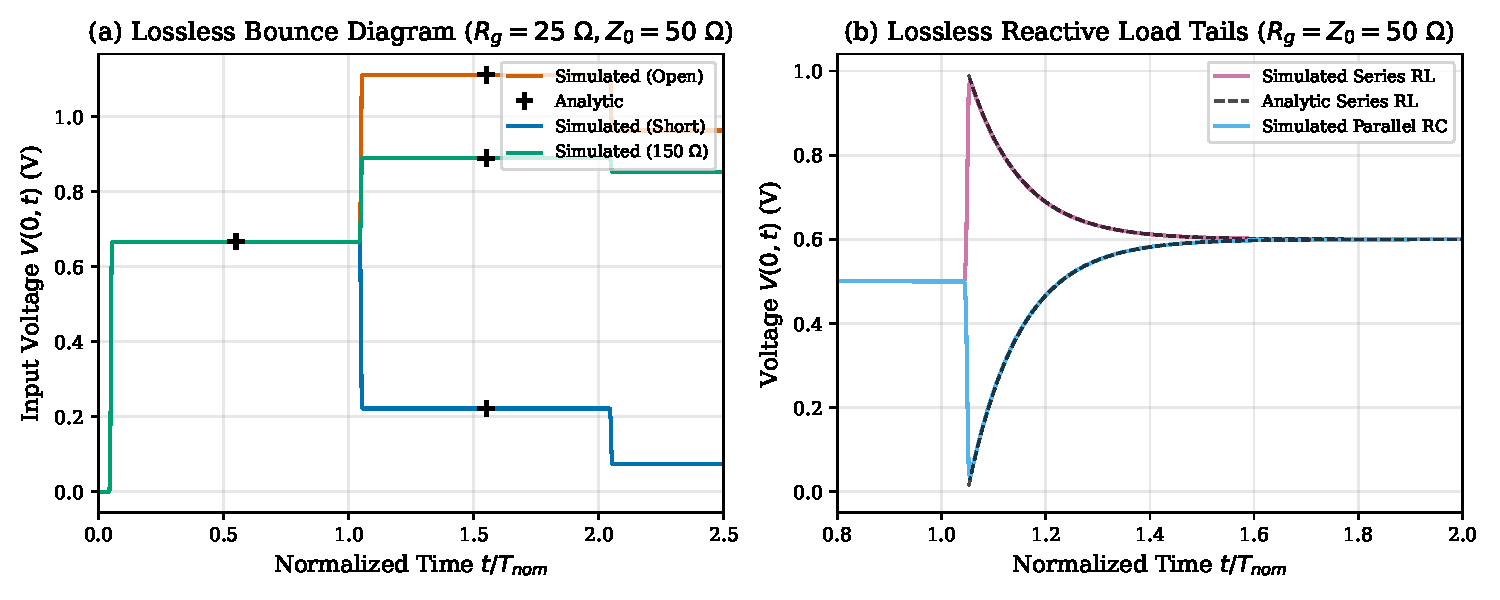
\includegraphics[width=\columnwidth]{fig_sim_validation.pdf}
\caption{Electromagnetic simulator validation: comparison against analytic lattice bounce diagrams on lossless lines ($R_g = 25\ \Omega$) and exact exponential transient tails for reactive $RL$ and $RC$ loads.}
\label{fig:sim_val}
\end{figure}

\begin{figure}[t]
\centering
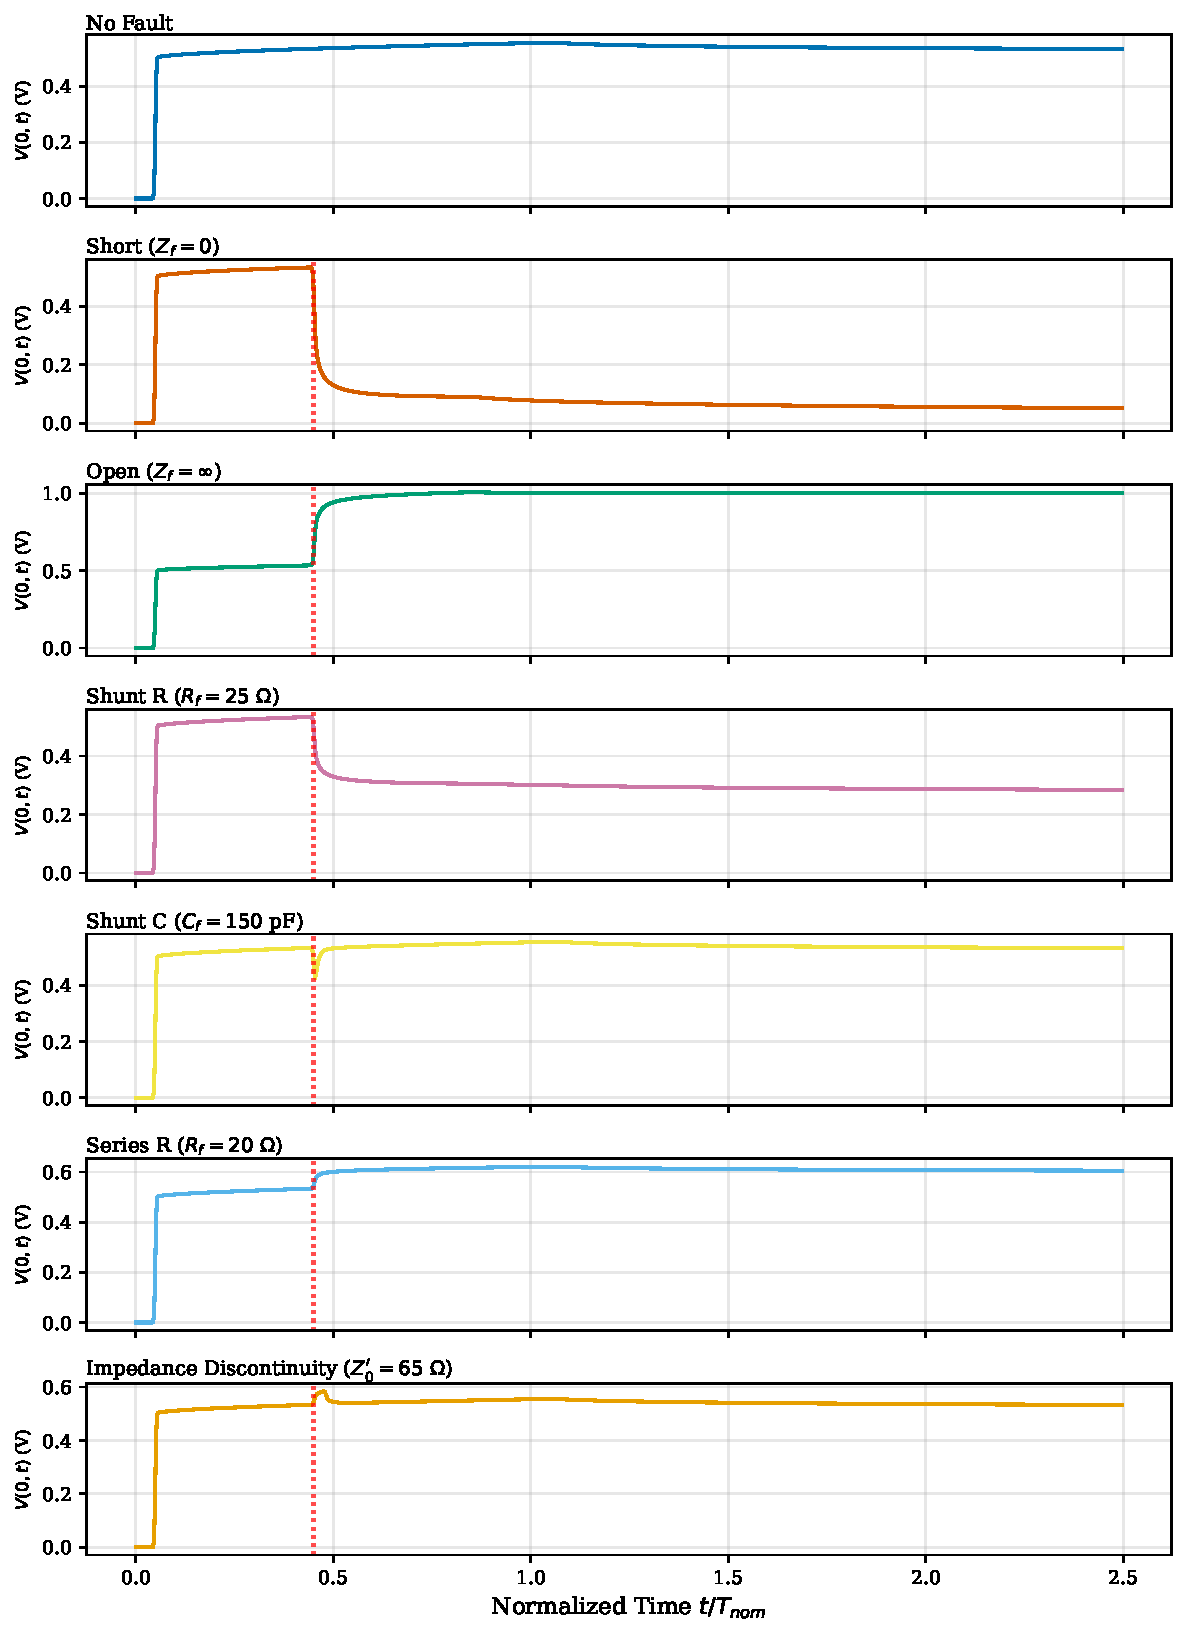
\includegraphics[width=\columnwidth]{fig_fault_gallery.pdf}
\caption{Exemplar clean TDR waveforms across the 7 fault classes for an identical cable geometry ($l = 100$~m, $d = 40$~m, matched termination).}
\label{fig:fault_gallery}
\end{figure}

\subsection{Dataset Formulation \& Out-of-Distribution Partitions}
The dataset is generated by independently sampling physical cable, fault and load configurations (all ranges are in \texttt{config.yaml}; ``log-uniform'' means uniform in the logarithm):
\begin{itemize}
    \item Cable length $l \in [20, 200]$~m; characteristic impedance $Z_0 \in [48, 52]\ \Omega$; velocity factor $v_f = 0.66\,\kappa$ with $\kappa \in [0.98, 1.02]$.
    \item Loss multiplier $s_{\mathrm{loss}} \in [0.7, 1.3]$ applied to $R_{dc}$ and $k_{\mathrm{skin}}$; generator rise time $t_r \in [1, 5]$~ns; source resistance $R_g \in [47.5, 52.5]\ \Omega$.
    \item Faults, balanced over the 7 classes, at $d/l \in [0.10, 0.95]$: shunt $R_f \in [5, 2000]\ \Omega$ and series $R_f \in [1, 200]\ \Omega$ (log-uniform); shunt $C_f \in [20, 500]$~pF (log-uniform); impedance section $Z_0' \in [35, 45] \cup [55, 70]\ \Omega$ with width $w \in [0.5, 3]$~m.
    \item Loads, balanced over the 6 classes: matched $R_L \in [49, 51]\ \Omega$; $R_L \in [5, 500]\ \Omega$ (log-uniform, with $[40, 62]\ \Omega$ excluded for the resistive class so that it is distinguishable from matched); reactive time constants $\tau/T_{\mathrm{nom}} \in [0.02, 0.3]$ (log-uniform).
    \item Measurement noise: white Gaussian with $\sigma = v_{\mathrm{inc}} 10^{-\mathrm{SNR}/20}$; during training the SNR is drawn uniformly in $[20, 50]$~dB for each trace.
\end{itemize}

The production corpus comprises:
\begin{itemize}
    \item \textbf{Training split:} 60,000 traces (seed 1).
    \item \textbf{Validation split:} 10,000 traces (seed 2), used for threshold tuning, early stopping, the learning curves and the ablations.
    \item \textbf{Test split:} 10,000 traces (seed 3), used for all headline results.
    \item \textbf{Out-of-distribution (OOD) subsets} ($5 \times 1{,}000$ traces, seed 4), each changing one factor beyond the training range:
    \begin{enumerate}
        \item \textit{Long cable:} $l \in [200, 300]$~m.
        \item \textit{High loss:} $s_{\mathrm{loss}} \in [1.5, 2.0]$.
        \item \textit{Impedance shift:} $Z_0 \in [44, 47] \cup [53, 56]\ \Omega$.
        \item \textit{Slow rise:} $t_r \in [5, 8]$~ns.
        \item \textit{Near load:} fault 0.3--3~m from the load (so $d/l$ can exceed the training maximum of 0.95); this subset contains no fault-free traces.
    \end{enumerate}
\end{itemize}
Generation is fully seeded and takes about 2~s per 1,000 traces (165~s for the full corpus). Fig.~\ref{fig:load_gallery} shows the six load signatures, Fig.~\ref{fig:loss_effect} the edge smearing caused by skin and dielectric loss as the cable gets longer, and Fig.~\ref{fig:noise_examples} one trace at three SNR levels.

\begin{figure}[t]
\centering
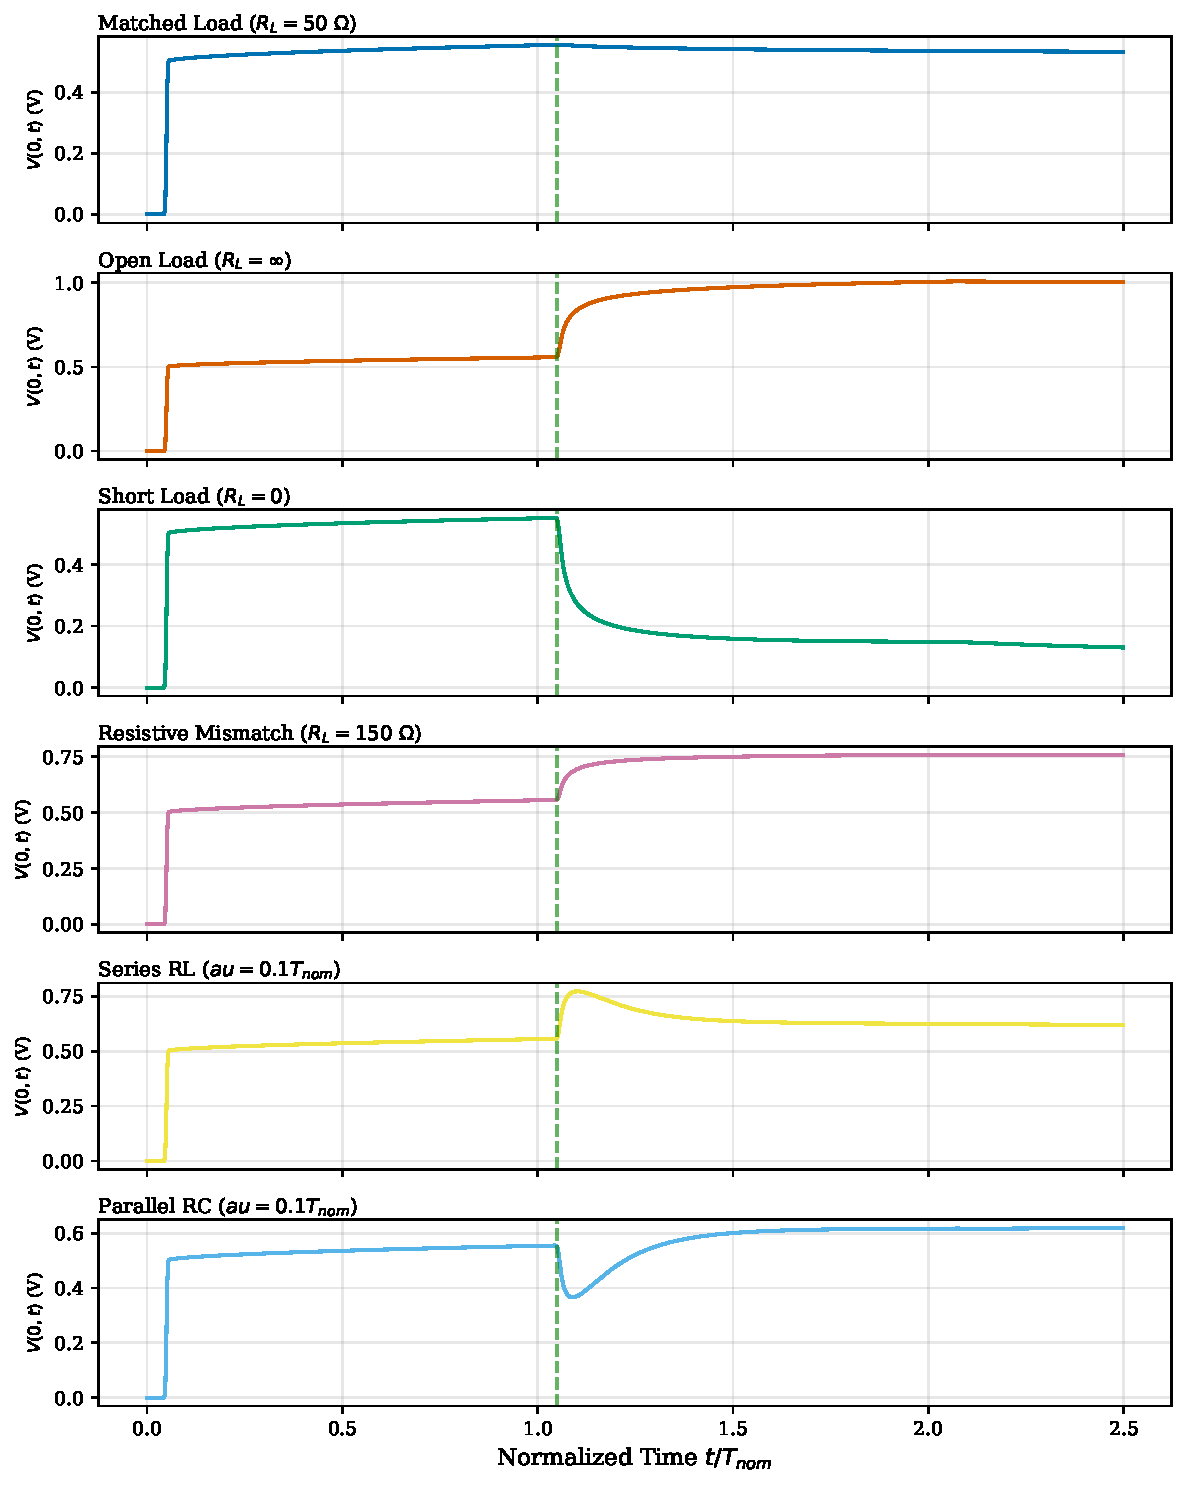
\includegraphics[width=\columnwidth]{fig_load_gallery.pdf}
\caption{Clean traces for the six load classes on a 100~m fault-free line. The dashed line marks the load echo; $RL$ and $RC$ loads produce exponential transients with time constant $\tau$.}
\label{fig:load_gallery}
\end{figure}

\begin{figure}[t]
\centering
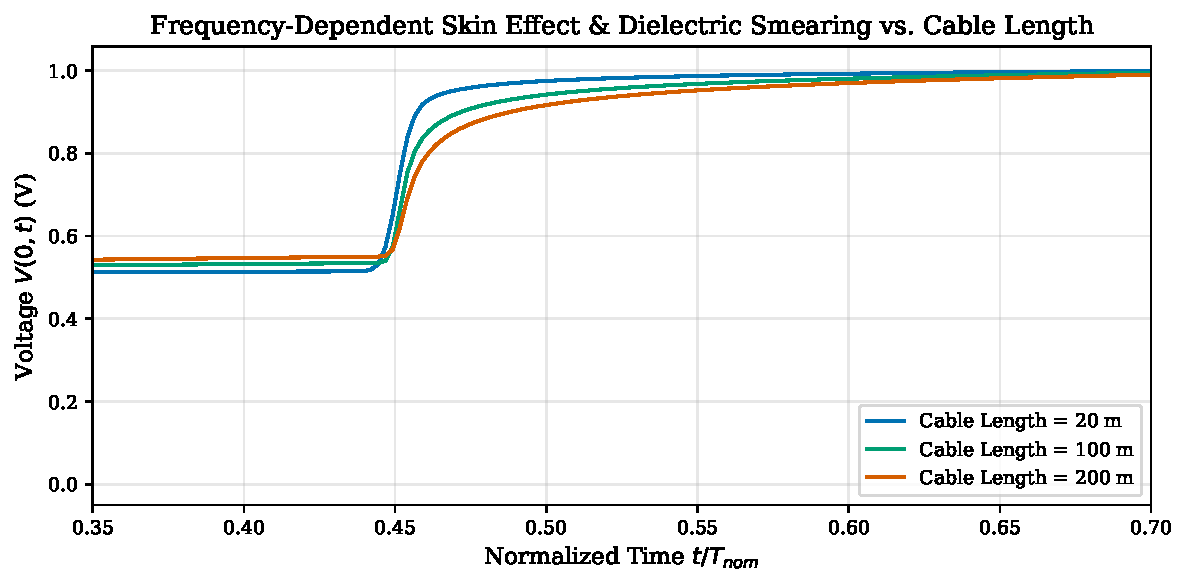
\includegraphics[width=\columnwidth]{fig_loss_effect.pdf}
\caption{Effect of conductor (skin) and dielectric loss: the open-load echo of a 20, 100 and 200~m cable, plotted on the normalised time axis. Longer cables give slower, more rounded edges.}
\label{fig:loss_effect}
\end{figure}

\begin{figure}[t]
\centering
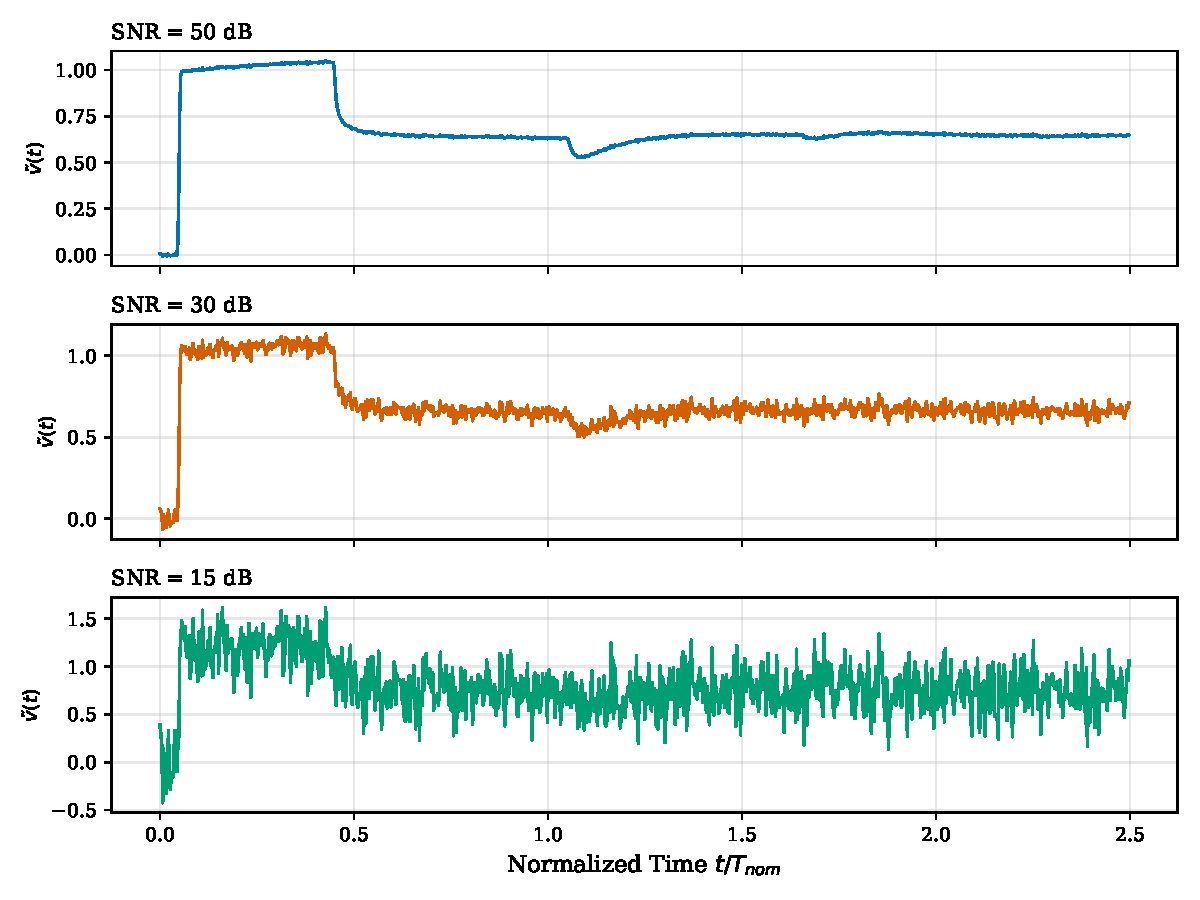
\includegraphics[width=\columnwidth]{fig_noise_examples.pdf}
\caption{The same trace (100~m line, $30\ \Omega$ shunt fault at 40~m, $RC$ load) at 50, 30 and 15~dB SNR, after normalisation.}
\label{fig:noise_examples}
\end{figure}

\subsection{Laboratory Dataset: WISE-CASING}
As a physical sanity check we use the public WISE-CASING laboratory TDR records \cite{nrel_wise_casing} (Lawrence Berkeley National Laboratory): an 80~m RG-85 coaxial cable with shorted termination, measured undamaged and with a $120^\circ$ shield cutaway at 40~m, plus records documented as 20, 10 and 5~m cables. These are \emph{pulse-type} reflectometry records (the signal returns to zero between echoes), not step responses, so the step-trained models are not applied to them. Instead we verify the propagation physics on real hardware: the velocity factor is estimated from the undamaged 80~m record, and the damage is located from the ratio of echo times (Section~\ref{sec:real_results}).

